\section{Hydrodynamik - Ideale Fluide (Reibungsfrei)}

\subsection{Kontinuitätsgleichung}

\begin{flushright}
	$\boxed{\textbf{Buch S. 166}}$
\end{flushright}

\begin{center}
	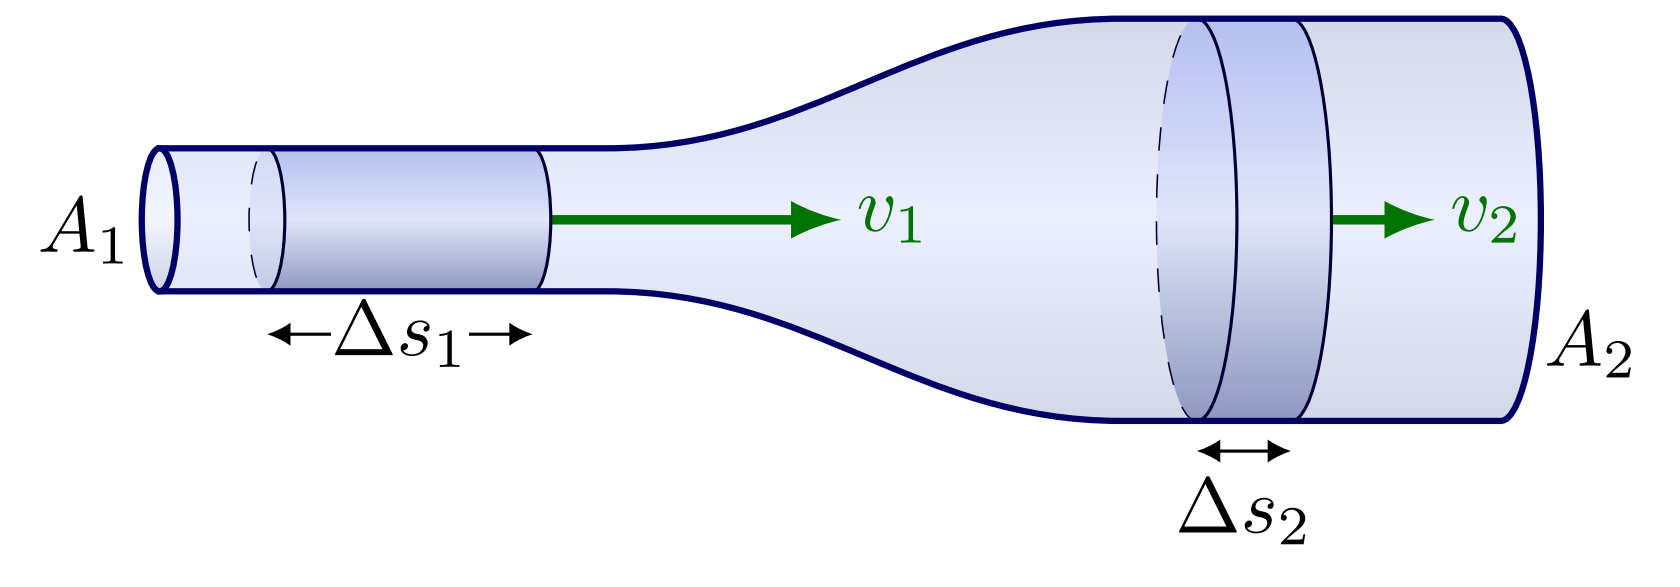
\includegraphics[width=0.7\columnwidth]{images/Kontinuitaet.png}
\end{center}

\vspace{-0.5cm}

$$ \boxed{ \frac{\Delta V}{\Delta t} = \dot{V} = A \cdot v = \const  \quad \Leftrightarrow \quad  A_1 \cdot v_1 = A_2 \cdot v_2 = \frac{\Delta V}{\Delta t} = \dot{V}} $$ 

\renewcommand{\arraystretch}{1.3}
\begin{tabular}{c l l}
	$\Delta V$	& Volumenänderung 					& $[\Delta V] = \meter^3$					\\
	$\Delta t$ 	& Zeitänderung 						& $[\Delta t] = \second$  					\\
	$\dot{V}$ 	& Volumenstrom (Volumen pro Zeit) 	& $[\dot{V}] = \frac{\meter^3}{\second}$	\\
	$A_x$ 		& Querschnittsfläche 				& $[A_x] = \meter^2$ 						\\
	$v_x$ 		& Geschwindigkeit der Flüssigkeit 	& $[v_x] = \frac{\meter}{\second}$
\end{tabular}
\renewcommand{\arraystretch}{1}

\medskip

\textrightarrow\ Gilt auch für Gase, wenn $v \ll v_{\rm Schall}$

\subsubsection{Massenstrom}


$$ \boxed{\dot{m} = \frac{dm}{dt} = \rho \cdot \dot{V}}$$

\begin{tabular}{c l l}
	$\dot{m}$ & Massenstrom  & $[\dot{m}] = \frac{\kilo \gram}{\second}$                   \\
	   $m$    & Masse        & $[m] = \kilo \gram$                             \\
	   $t$    & Zeit         & $[t] = \second$                              \\
	 $\rho$   & Dichte       & $[\rho] = \frac{\kilo \gram}{\meter^3}$              \\
	$\dot{V}$ & Volumenstrom & $[\dot{V}] = \frac{\meter^3}{\second}$
\end{tabular}


\subsection{Bernoulli-Gleichung}

\begin{flushright}
	$\boxed{\textbf{Buch S. 168}}$
\end{flushright}

\subsubsection{Hydrodynamisches Paradoxon}

$\Rightarrow$ Je \textbf{grösser} die \underline{Strömungsgeschwindigkeit}, desto \textbf{kleiner} der \underline{Druck}

\subsubsection{Kräftegleichgewicht}

\begin{minipage}[c]{0.38\columnwidth}
	\raggedright
	Die Bernoulli-Gleichung beschreibt ein \myul{bewegtes} Fluid

	$$ \underbrace{ p + \rho \cdot g \cdot h }_{\substack{\mathrm{statisch}}} 
	+ \underbrace{ \frac{1}{2} \, \rho \cdot v^2 }_{\substack{\mathrm{dynamisch}}} = \const $$
\end{minipage}
\hfill
\begin{minipage}[c]{0.6\columnwidth}
	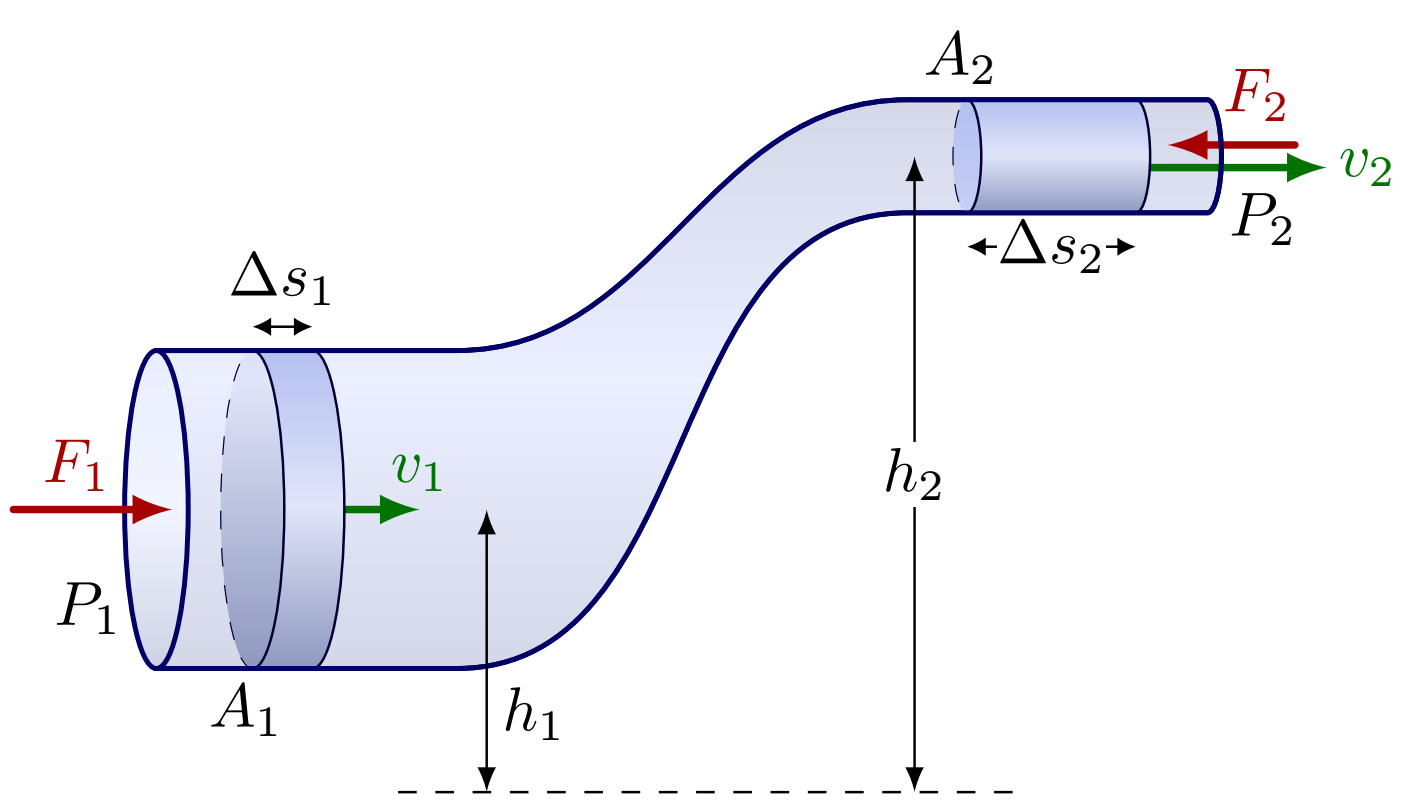
\includegraphics[width=\columnwidth]{images/Bernoulli.png}
\end{minipage}

\smallskip

$$ \boxed{ p_1 +  \rho \cdot g \cdot h_1 + \frac{1}{2} \, \rho \cdot v_1^2 = p_2 +  \rho \cdot g \cdot h_2 + \frac{1}{2} \, \rho \cdot v_2^2 } $$


\begin{tabular}{c l l}
	$p_x$  & Druck in der jeweiligen Position & $[p] = \pascal = \bbar$   \\
	$\rho$ & Dichte Flüssigkeit / Gas         & $[\rho] = \frac{kg}{m^3}$ \\
	 $g$   & Erdbeschleunigung                & $[g] = \frac{m}{s^2}$     \\
	$h_x$  & Höhe der Position                & $[h] = m$                 \\
	$v_x$  & Geschwindigkeit des Mediums      & $[v] = \frac{m}{s}$
\end{tabular}

\subsection{Spezialfälle - Umformungen}
\begin{flushright}
	$\boxed{\textbf{Buch S. 165 \& 168}}$
\end{flushright}

\begin{minipage}[t]{0.48\columnwidth}
	\subsubsection{Spezialfall: Horizontal}

	$$ \boxed{ p + \frac{1}{2} \, \rho \cdot v^2 = \const } $$
\end{minipage}
\hfill
\begin{minipage}[t]{0.48\columnwidth}
	\subsubsection{Spezialfall: Statik}

	$$ \boxed{ p + \rho \, \cdot g \cdot h =  \const} $$
\end{minipage}


\subsubsection{Spezialfall: Torricelli}

$$ \boxed {v=\sqrt{2 \cdot g \cdot h}}$$

\begin{tabular}{c l l}
	$v$ & Ausflussgeschwindigkeit & $[v] = \frac{m}{s}$   \\
	$g$ & Erdbeschleunigung       & $[g] = \frac{m}{s^2}$ \\
	$h$ & Höhe der Flüssigkeit    & $[h] = m$
\end{tabular}

\subsubsection{Volumenstrom in Kombination mit Bernoulli}

$$ \boxed{\dot{V} = A_1 \sqrt{\frac{2 \Delta p}{\rho \left[ \left( \frac{A_1}{A_2} \right)^2 - 1 \right]}}}$$

\begin{tabular}{c l l}
	$\dot{V}$  & Volumenstromfluss, alternativ $Q$ & $[\dot{V}] = \frac{m^3}{s}$    \\
	$\Delta p$ & Druckdifferenz                    & $[\Delta p] = \pascal = \bbar$ \\
	  $A_x$    & Querschnittsfläche                & $[A] = m^2$                    \\
	  $\rho$   & Dichte Flüssigkeit                & $[\rho] = \frac{kg}{m^3}$
\end{tabular}
\vspace{0.2cm}
\begin{itemize}
	\item nur möglich in einem abgeschlossenen Rohrsystem 
	\item wenn $\rho$ gleich bleibt = konst.
\end{itemize}

\subsection{Bernoulli-Gleichung und Energieerhaltung}

Die in der Bernoulli-Gleichung vorkommenden Terme können als \myul{Energie pro Volumen} betrachtet werden.

\vspace{-0.3cm}

\begin{align*}
	E_{\rm Mech}	&= \text{Elastische Energie } + \text{ pot. Energie } + \text{ kin. Energie} \\
					&= p \cdot V + m \cdot g \cdot h + \frac{1}{2} \, m \cdot v^2 = \const
\end{align*}



Wenn durch das Volumen dividiert wird erhält man: 

\vspace{-0.3cm}

\begin{align*}
	\frac{E_{\rm Mech}}{\text{Volumen}}	&= \frac{\text{elatische Energie}}{\text{Volumen}} + \frac{\text{pot. Energie}}{\text{Volumen}} + \frac{\text{kin. Energie}}{\text{Volumen}} \\
										&= p + \rho \cdot g \cdot h + \frac{1}{2} \, \rho \cdot v^2 = \const
\end{align*}


Bei einer horizontalen Strömung entfällt die pot. Energie (pro Volumen)

\vspace{-0.3cm}

\begin{align*}
	\frac{E_{\rm Mech}}{\text{Volumen}}	&= \frac{\text{elatische Energie}}{\text{Volumen}} + \frac{\text{kin. Energie}}{\text{Volumen}} \\
										&= p + \frac{1}{2} \, \rho \cdot v^2 = \const
\end{align*}

\subsection{Pumpenleistung}

$$ \boxed {P= \frac{W}{t} = p \cdot \dot{V} = p \cdot A \cdot v}$$

\begin{tabular}{c l l}
	$P$ & Leistung & $[P] = \frac{\joule}{\second} = \watt $   \\
	$p$ & Druck       & $[p] = \frac{\newton}{\meter^2} = \pascal$ \\
	$\dot{V}$ & Volumenstrom   & $[\dot{V}] = \frac{\meter^3}{\second}$
\end{tabular}

